\documentclass[10pt,conference,compsocconf]{IEEEtran}

\usepackage{hyperref}
\usepackage{graphicx}	% For figure environment


\begin{document}
\title{Higgs Boson Challenge}

\author{
  Ignacio Aleman, Thierry Bossy, Raphael Strebel\\
  \textit{EPFL, Lausanne}
}

\maketitle

\begin{abstract}
The Higgs Boson challenge is one of the most popular Machine Learning competitions. Based on simulations done in the ATLAS Experiments, the goal is to find out whether or not key signatures of the Higgs Boson are present. In this paper, we tackle this binary classification task by preprocessing the data and applying basic ML methods such as regression. The best solution we find consists of partitioning the input data according to one specific experiment measure and training independent models for each partition. From the results we conclude that this method performs fairly well. Indeed, we classify correctly around 83\% of the test data.

\end{abstract}

\section{Introduction}

In 1964, Peter Higgs -- amongst others -- theorized the existence of a mechanism that gave mass to matter, the Higgs mechanism. In turn, this mechanism implied the presence of the Higgs Boson. To confirm this -- as well as other fundamental theories -- CERN was established, and in 2012 the ATLAS and CMS both independently managed to show the presence of the Higgs Boson.

The idea was simple, to collide particles at high speeds and to capture key signatures during the collision. Then the question to be answered was, given the observed signatures, can we conclude the presence of the Higgs Boson?

The Higgs Boson Machine Learning Challenge was designed to classify the characterizing events in order to deretmine the presence of the tau decay of a Higgs Boson. 

To get a better picture of the data, we went over the official review of the challenge \cite{higgsPaper} which gives useful information on the acquisition of the data. For example it explains why certain values are missing, which gives an idea as to how it might be worth to split the data. In the following we describe our approach to this challenge, starting with the preprocessing of the data. We then explain which models we choose and conclude by analysing the results we obtain. Finally we give an brief overview of other methods that could be tried to improve the performance of the model.

\section{preprocessing}

\label{sec:preprocessing}
Preprocessing is an essential step that allows us to considerably improve the result given by our model. This is even more the case as we only used basic techniques in this project, as opposed to neural networks. By inspecting the shape of the data and the role of certain features, some steps can be applied before feeding our model with the data.

\subsection{Jet number}

From \cite{higgsPaper} we found out that the \textit{jet\_number}, a feature of the data, directly implies values of certain features of our data to be undefined, in particular the following are undefined for each jet num.

\begin{itemize}
  \item If jet num = 0: PRI jet leading pt, PRI jet leading eta, PRI jet leading phi are undefined
  \item If jet num $\leq$ 1: DER deltaeta jet jet, DER mass jet jet, DER prodeta jet jet, DER lep eta centrality, PRI jet subleading pt, PRI jet subleading eta, PRI jet subleading phi are undefined.
\end{itemize}

This means that by splitting the input $X$ based on the jet number, we can remove certain feature columns the data in each subset. As the jet number can only take values in the set $\{0,1,2,3\}$, and as a value of 2 or 3 makes no difference on the implications of other features, we divide $X$ into $\{X_0,X_1,X_{2,3}\}$. We then remove the features of those subsets accordingly, as well as the column that contains the jet number in all subsets of $X$ since we no longer need it. See Figure~\ref{fig:jet-split} for a more visual explanation.

\begin{figure}[h]
  \centering
  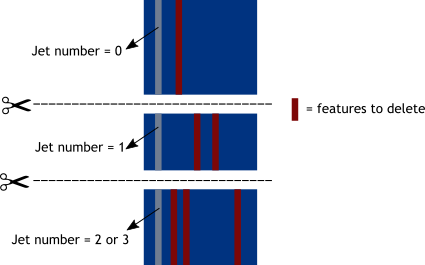
\includegraphics[width=\columnwidth]{jets.png}
  \caption{Splitting the data samples according to jet number}
  \vspace{-3mm}
  \label{fig:jet-split}
\end{figure}

\subsection{Undefined values}

Probably because of erroneous measurements, the input still contains undefined values even after the previous simplification. To deal with this issue, we replace undefined values of a feature by the mean of the feature. (We also tried the mode and median, but found the mean to give the best results).

\subsection{Standardisation}

To standardise the features of the data, we determine the mean and the variance of every column, and normalize each column of the input by subtracting its mean and dividing by its standard deviation. 

\subsection{Feature augmentation}

After cleaning the data we get a good boost in accuracy (we go from .62 to .78). In order to go beyond that, we tried feature augmentation. The idea is, of course, that if we choose a rich enough representation, we are able to find some higher dimensional space where the data is linear.

First of all, we add a bias $1$ column to our input based on our intuition for simple linear models. Next, we tried to compute polynomials of our data and consider them as new features. We continue the process by computing all cross-products of the columns of $X$ and, as before, consider them as new features. This roughly squares the dimension of each subset $X_i$, which is already much better. Next, we apply a hyperbolic tangent function to our initial features so that the result is normalized in the domain $]-1, 1[$ and does not penalize outliers too greatly as explained in \cite{normTechniques}. The final data augmentation we do is to give the option of combining the previously described functions. Indeed, instead of computing only functions of the initial features, we can get a much richer model if we choose to compute functions of the previously determined features. For example, we could compute the polynomials of degrees 2 and 3 of an input $X$, then we can compute the $tanh$ of each column and append the result to the data. If we wanted to go even further, we could also compute the cross-product of all previously determined columns and consider them as part of the augmented data.

We found one of the biggest boost in accuracy by not only considering the cross terms of the data, but also by looking at the cross terms of polynomials. (Indeed this allows to represent a richer function).

\section{Models}

We first tried both standard regression as well as logistic regression, and we found that using standard regression far outperformed logistic regression. We thus decided to go for standard regression, and to try and control over-fitting we choose to go for ridge regression (though we found that $\lambda$, the $L_2$ penalty, had little influence).

Thus, in essence our model selection process consisted in finding the right combination of feature augmentation. Recall that we split out data -- based on the jet number -- into 3 sets ($X_0$, $X_1$ and $X_{2,3}$).

For each subset of the data, we tried to find the right combination of feature augmentation (see \ref{table:1}) to maximise the predictive accuracy. 
 
\begin{table}[h!]
\centering
\begin{tabular}{||c c c c c c||} 
 \hline
 Data & Degree & Bias & Cross & Tanh & Cumulative\\ [0.5ex] 
 \hline\hline
 $X_0$ & [2, 3] & yes & yes & yes & no \\ 
 $X_1$ & [2] & yes & yes & yes & yes \\
 $X_2,_3$ & [2] & yes & yes & yes & yes \\

 \hline
\end{tabular}
\caption{Table of chosen data augmentation per data split}
\label{table:1}
\end{table}


\section{Results}

With the aforementioned model we found an accuracy of \textbf{0.829} on the test set via the \textbf{AI crowd portal}. Before evaluating on the challenge test set, we split our own train data into a resp. test/split set to check the accuracy. We performed 10 random splits to get an idea of the variance of our accuracy. We describe the result -- also per jet num -- in Table \ref{table:2}. We see that our model performs quite well for jet num 0 and 2, 3, but not so well for jet num 1.

\begin{table}[h!]
\centering
\begin{tabular}{||c c||} 
 \hline
 Dataset & Accuracy \\ [0.5ex] 
 \hline\hline
 $X_0$ & 0.841 +- 0.004  \\ [0.5ex] 
 $X_1$ & 0.819 +- 0.005 \\[0.5ex] 
 $X_2,_3$ & 0.850 +- 0.002 \\[0.5ex] 
 \hline\hline
 $X$ & 0.837 +- 0.002 \\

 \hline
\end{tabular}
\caption{Model accuracy per data split}
\label{table:2}
\end{table}
\section{Discussion}

Surprisingly a linear model worked better than a fancier logistic regression. However, we did not try to optimise the data augmentation for the logistic model, so the aforementioned claim should be taken with a grain of salt.

Apart from feature augmentation, we also tried to perform
PCA on the data, however we did not find any sort of gain and therefore did not follow this direction further.

Clearly finding the right and large enough feature augmentation technique gave the largest improvement in accuracy.

\section{Future work}

In line with the previous discussion, the authors believe that a more through search of feature augmentation should further allow to increase the accuracy. (e.g. Kernel methods)


\bibliographystyle{IEEEtran}
\bibliography{literature}

\end{document}
